\tikzsetnextfilename{caseC_iterations}
\begin{figure}[ht]
\centering
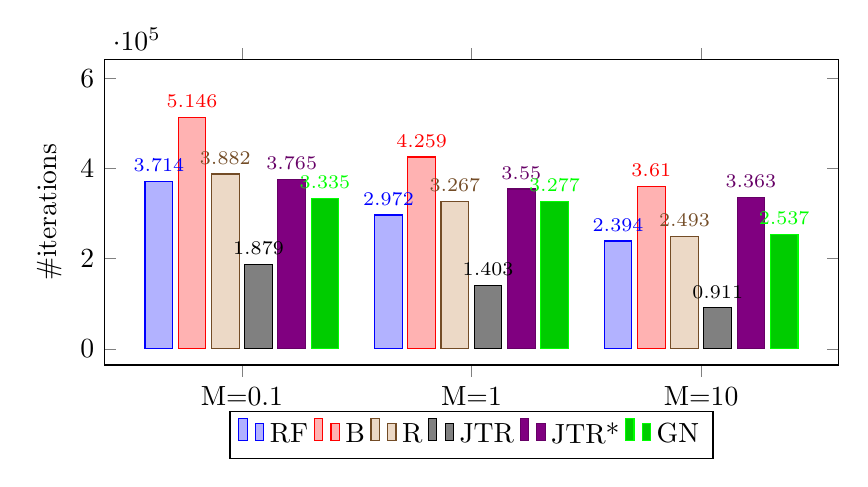
\begin{tikzpicture}
\begin{axis}[
    width=0.9\textwidth,
    height=0.45\textwidth,
    ybar,
    enlargelimits=0.3,
    legend style={at={(0.5,-0.15)},
      anchor=north,legend columns=-1},
    ylabel={\#iterations},
    symbolic x coords={M=0.1,M=1,M=10},
    xtick=data,
    nodes near coords,
    every node near coord/.append style={
    	font=\scriptsize,
	/pgf/number format/precision=3},
    point meta=y *10^-5
    ]
\addplot coordinates {(M=10,239352) (M=1,297199) (M=0.1,371414)};
\addplot coordinates {(M=10,360967) (M=1,425877) (M=0.1,514572)};
\addplot coordinates {(M=10,249254) (M=1,326676) (M=0.1,388250)};
\addplot coordinates {(M=10,91061) (M=1,140320) (M=0.1,187857)};
\addplot coordinates {(M=10,336270) (M=1,355013) (M=0.1,376547)};
\addplot coordinates {(M=10,253670) (M=1,327701) (M=0.1,333513)};
\legend{RF,B,R,JTR,JTR*,GN}
\end{axis}
\end{tikzpicture}
\caption{Number of iterations spent for six different root finders when solving Case C, see Section \ref{section:caseA}, with viscosity ratio $M = \frac{\mu_w}{\mu_o}$. Root finders: RF (Regula Falsi), B (Brent), R (Ridders), JTR (Jenny Trust Region), JTR* (Approximate Jenny Trust Region), and GN (Globalized Newton).}
\label{fig:caseC_iterations}
\end{figure}